%%%%%%%%%%%%%%%%%%%%%%%%%%%%%%%%%%%%%%%%%%%%%%%%%%%%%%%%%%%%%%%%%%%%%%%%%%%%%%%%
%2345678901234567890123456789012345678901234567890123456789012345678901234567890
%        1         2         3         4         5         6         7         8

\documentclass[letterpaper, 10 pt, conference]{ieeeconf}  % Comment this line out if you need a4paper

%\documentclass[a4paper, 10pt, conference]{ieeeconf}      % Use this line for a4 paper

\IEEEoverridecommandlockouts                              % This command is only needed if 
                                                          % you want to use the \thanks command

\overrideIEEEmargins                                      % Needed to meet printer requirements.
\pdfminorversion=4
% See the \addtolength command later in the file to balance the column lengths
% on the last page of the document

% The following packages can be found on http:\\www.ctan.org
\usepackage{graphics} % for pdf, bitmapped graphics files
\usepackage{graphicx}
%\usepackage{epsfig} % for postscript graphics files
%\usepackage{mathptmx} % assumes new font selection scheme installed
%\usepackage{times} % assumes new font selection scheme installed
\usepackage{amsmath} % assumes amsmath package installed
\usepackage{float}
%\usepackage{amssymb}  % assumes amsmath package installed
\usepackage[x11names]{xcolor}
% Uncomment the following line and comment the one after to obtain the final version without comments
\usepackage[draft]{changes} 

\definechangesauthor[color=red]{jeg}
\definechangesauthor[color=magenta]{fra}
\definechangesauthor[color=RoyalBlue3]{nav}

\title{\LARGE \bf
Extended Kalman Filter Based Estimation of Dynamic Quantities and Stability Indices for Bipedal Posture Control}

\author{Jorhabib Eljaik, Naveen Kuppuswamy and Francesco Nori% <-this % stops a space
\thanks{*This paper was supported by the FP$7$ EU projects CoDyCo (No. $600716$ ICT $2011.2.1$ Cognitive Systems and Robotics), and Koroibot (No. $611909$ ICT-$2013.2.1$ Cognitive Systems and Robotics). }% <-this % stops a space
\thanks{Authors are with the Department of Robotics, Brain, ad Cognitive Sciences (RBCS) at the Istituto Italiano di Tecnologia, via Morego 30, Genova Italy.  ({email : \tt\small \{francesco.nori,jorhabib.eljaik, naveen.kuppuswamy\} @ iit.it}}%% \thanks{$^{2}$Bernard D. Researcheris with the Department of Electrical Engineering, Wright State University,
%         Dayton, OH 45435, USA
%         {\tt\small b.d.researcher@ieee.org}}%
 }

\begin{document}



\maketitle
\thispagestyle{empty}
\pagestyle{empty}

%%%%%%%%%%%%%%%%%%%%%%%%%%%%%%%%%%%%%%%%%%%%%%%%%%%%%%%%%%%%%%%%%%%%%%%%%%%%%%%%%%
\begin{abstract}
 We have designed and implemented and Extended Kalman Filter (EKF) that integrates force/torque (FT) measurements from the leg and ankle of a humanoid robot with readings from an accelerometer placed on its foot and the dynamic model of its leg to estimate different dynamic quantities. The FT measurements in the thigh can be seen as a replacement of the dynamics of the rest of the body. The main contributions are in the usage of rigid body dynamics for state update and the incorporation of control variables $u$ within the state update, thus allowing the EKF to estimate external wrenches based based also on their direct or indirect measurement.
 \end{abstract}
 
\begin{keywords}
 Extended Kalman Filter, dynamic quantity estimation, sensor fusion, stability measuremens, balance, foot rotation indicator, center of pressure.
\end{keywords}



%%%%%%%%%%%%%%%%%%%%%%%%%%%%%%%%%%%%%%%%%%%%%%%%%%%%%%%%%%%%%%%%%%%%%%%%%%%%%%%%%%
\section{INTRODUCTION}
% \added[id=fra]{FRA This introduction still sucks, cause I've been pretty much putting loose paragraphs and ideas. They're not all very well connected. It still needs some work. Something you could really help me us with here is to elaborate a little bit more on the references and state of the art. See my comments in the last paragraphs. Moreover, when it comes to the contributions of this work, I remember it was very clear for you what was interesting about this work with respect to previous ones, even though it is fairly simple.}
The evolution of a technological world built for and by humans comes with a continuing demand for machines that are also able to assist us in a more human-like fashion. To this end, bipedal humanoid robots are thought of as the perfect tool, and to be such, these machines must move as we do in our unstructured environment and \emph{interact} with it while accounting for \emph{whole-body postures}. The coexistence of these last two aspects implies that bipedal robots must be able to balance while in multiple contacts, which in turn means, that  the wrenches due to contacts ($f_c$, $\mu_c$) and those due to the movement of the body ($f_o$, $\mu_o$) must balance. Basic stability criteria for bipedal robots are based on this principle and a first introduction of such concept was done in \cite{Vukobratovic1969} by Vukobratovic et al. who defined the \emph{zero moment point} (ZMP) as a unique point on the ground where $f_c$, $\mu_c$ produce zero tangential moments while the corresponding sability criterion considered that this point should stay away from the border of the convex hull of both feet in contact with the ground.

Goswami in \cite{Goswami1999} pointed out that the ZMP-based stability criterion is limited for gait planning. He therefore formulated some different statements for the characterization of the stability of planar unilateral contacts. These statements made use of the \emph{foot rotation indicator} (FRI) which corresponds to the unique zero tipping moment point associated to $f_o$, $\mu_o$ and belongs to the contact plane. The FRI can however move outside the convex hull meaning that a rotation of the foot is happening and thus allowing the distinction between a marginal state of static equilibrium and loss of balance. 

\section{State of the art and beyond}

Several authors have used either the ZMP or the FRI for gait planning, mostly relying on force/torque (FT) sensors at the ankles or sensor arrays at the feet soles. These sensors allow only an instantaneous measurement of the ZMP and therefore several authors have suggested the use of a Kalman filter \cite{KalmanDeSchutter} to improve the signal to noise ration and, more interestingly, to predict the ZMP position by exploiting its dynamics as it results from the integration of the whole body dynamics. 

Kalman filter based ZMP estimation has been used in \cite{Park2007}, where authors proposed a three dimensional linear inverted pendulum model to filter the measured ZMP position and to get a more reliable measurement for achieving stable walking. More recently, Park et al. \cite{park2009balance} introduced an estimation procedure which uses camera images to filter the robot pose and to get a Kalman filter estimation of the ZMP position.

In this paper we present a framework for obtaining estimates of the dynamic quantities necessary for the computation of stability measurements (ZMP or FRI) through an Extended Kalman Filter (EKF) based data fusion approach. The main contributions are in the usage of rigid body dynamics for state update and the incorporation of control variables $u$ within the state update, thus allowing the EKF to estimate external wrenches based also on their direct or indirect measurement. We have designed and implemented and EKF that integrates multiple F/T measurements with readings from an accelerometer placed on the foot and the dynamic model of the leg to estimate different dynamic quantities. The EKF uses an augmented state vector to include the applied wrenches and foot orientation (after local parametrization). Our approach instead uses FT sensors and accelerometers along with the dynamic model of the leg to estimate (among other quantities) contact and inertial forces that will then allow us to have a more reliable stability measurement. It is worth noting that this framework could then be extended to the rest of the body when external forces occur at points different from the feet soles. 

The structure of the paper is as follows. In Section \ref{section:framework} the proposed framework is explained, starting from the dynamic model of a general rigid body system subject to two measureable external wrenches and with a single measurement of linear acceleration. A brief introduction to the Extended Kalman Filter and later explained how the estimated external wrenches can be used for better estimation of different stability measurements, in particular, FRI and COP. Section \ref{section:experiments} contains details about the simulated and real setups as well as the specificities of the platform and the obtained results, while Section \ref{section:conclusions} draws some conclusions and analysis of the obtained results. Finally, Section \ref{section:futureWork} elaborates on the enhancemens that can be done and how we plan to scalate the framework to estimate dynamic quantities for the entire body of the robot and ideas on how to make this efficiently.

% \added[id=jeg]{Some keywords to remember: Sensor fusion, dynamic model; Importance of dynamic estimation for better control algorithms; Importance of a good balance indicator (stress out the importance of using the FRI as opposed to CoP, etc); Importance of the Extended Kalman Filter; What's interesting about our approach; Structure of the paper}

% Kinematic calibration. Stochastic framework (graphical models). EM-like optimization \cite{Wu2013}.
% 
% 
% a preliminary version which claims to use system dynamics (and indeed dynamic quantities are considered) \cite{Lowrey2014}.
% 
% decoupled floating base and joint EKF. Kinematic constraints explicitly modeled and assumed as rigid contacts \cite{Xinjilefu2014}.
% 
% LIMP simplified model. Taxonomy of different models (with or without external force, with or without COM offset) \cite{Stephens2011}.
% 
% Comparison between LIMP model and full model. Interesting digression on KF with state constraints (model reduction, estimate projection) \cite{Xinjilefu2012} . Slipping detection is underlined as a fundamental issue and two approaches proposed \cite{Okita2012}, \cite{Kaneko2005}.
% 
% Pose and footprints estimation for quadrupeds. Footprints are included in the state space. Estimation of noise variance with Allan variances. Multiplicative representation of orientation. Observability analysis. 
% 
% \cite{Bloesch2012}

%%%%%%%%%%%%%%%%%%%%%%%%%%%%%%%%%%%%%%%%%%%%%%%%%%%%%%%%%%%%%%%%%%%%%%%%%%%%%%%%%%
\section{PROPOSED FRAMEWORK}
\label{section:framework}
% \added[id=jeg]{JORHABIB: Explain first in general basic concept of Kalman and extended Kalman filter including also the equations. Check other papers to see how much in detail they go. Then pass to general descritpion of the framework for a rigid body system and it can then be used with the extended kalman filter, pointing out the expansion of the state vector to include external wrenches and local parametrization}

\subsection{Extended Kalman Filter}
\label{subsection:extended-kalman-filter}
The Kalman Filter is a tool for stochastic data fusion in which the state of a system is estimated, based on measurements of the system and its linear model. It minimizes in the least squares sense the inconsistencies with all pieces of information available to obtain the best estimate possible. Measurements and state estimates are expressed as Gaussian distributions thus allowing to express a desired level of confidence on the information. The model of the system consists of a \emph{state equation}, a \emph{measurement equation}, the measurement and process \emph{covariance matrices} $R$ and $Q$, and the \emph{initial state estimate} $\hat{x}_0$ with its corresponding initial covariance matrix $\hat{P}_0$.

The differentiable state transition and observation models that are used in the EKF are expressed as: 

\begin{align}
 x_k &= f(x_{k-1}, u_{k-1}) + w_{k-1} \\
 y_k &= h(x_k) + v_k
\end{align}

Where $x_k$ is the state vector at time $k$, $f$ is the nonlinear state function, $u$ the control input. $y_k$ is the observation at time $k$ with measurement prediction function $h$. The process noise $w$ and the observation noise $v$ have Gaussian distributions $\mathcal{N}(0,\sigma_w^2)$ and $\mathcal{N}(0,\sigma_v^2)$ respectively with corresponding covariance matrices $Q_k = \sigma_w^2 \mathbf{I}_{n\times n}$ and $R_k = \sigma_v^2 \mathbf{I}_{m\times m}$, where $n$ is the dimension of the state vector and $m$ of the measurement vector.

When the measurement and state equations are nonlinear, these can be linearized about the most recent state estimate in order to apply the Kalman Filter. This is known as the Extended Kalman Filter, which consists of a \emph{prediction} and an \emph{update} stage with the following equations:

\subsubsection{Prediction} 
\begin{itemize}
\item State prediction: $\tilde{x}_{k|k-1} = f(\hat{x}_{k-1|k-1})$
\item Covariance prediction: $\tilde{P}_{k|k-1} = F_{k-1}\hat{P}_{k-1|k-1}F^T_{k-1} + Q_{k-1}$ 
\end{itemize}

\subsubsection{Update}
\begin{itemize}
 \item State estimate: $\hat{x}_{k|k} = \tilde{x}_{k|k-1} + K_k (y_k - h(\tilde{x}_{k|k-1}))$
 \item Covariance matrix estimate: $\hat{P}_{k|k} = (I - K_k H_k) \tilde{P}_{k|k-1}$
\end{itemize}

Where $\tilde{\cdot}$ stands for prediction and $\hat{\cdot}$ for estimate. The subscript $k|k-1$ indicates a computation at time $k$ given others at time $k-1$ and similarly for $k-1|k-1$ and $k|k-1$. $P$ and $Q$ are the state and noise covariance matrices respectively. $F_{k-1}$ is the state transition matrix, computed as the Jacobian of the state function evaluated at the previous state estimate, i.e. $\frac{\partial f}{\partial x} \rvert_{\hat{x}_{k-1|k-1}}$.

In the update equations $K_k$ is the Kalman gain and can be obtained as $K_k = \tilde{P}_{k|k-1} H^T_k S^{-1}_k$, where $H$ is the observation matrix, computed as the Jacobian with respect to the state vector of function $h$, i.e. $H_k = \frac{\partial h}{\partial x} \rvert_{\tilde{x}_{k|k-1}}$, while $S$ is the residual covariance matrix computed as $S_k = R_k + H_k \tilde{P}_{k|k-1} H^T_k$.

The transition and observation models will come from the dynamic model of a rigid foot in contact with the ground as described next.

\subsection{Dynamic model}

\begin{figure}[htb]  
  \centering
    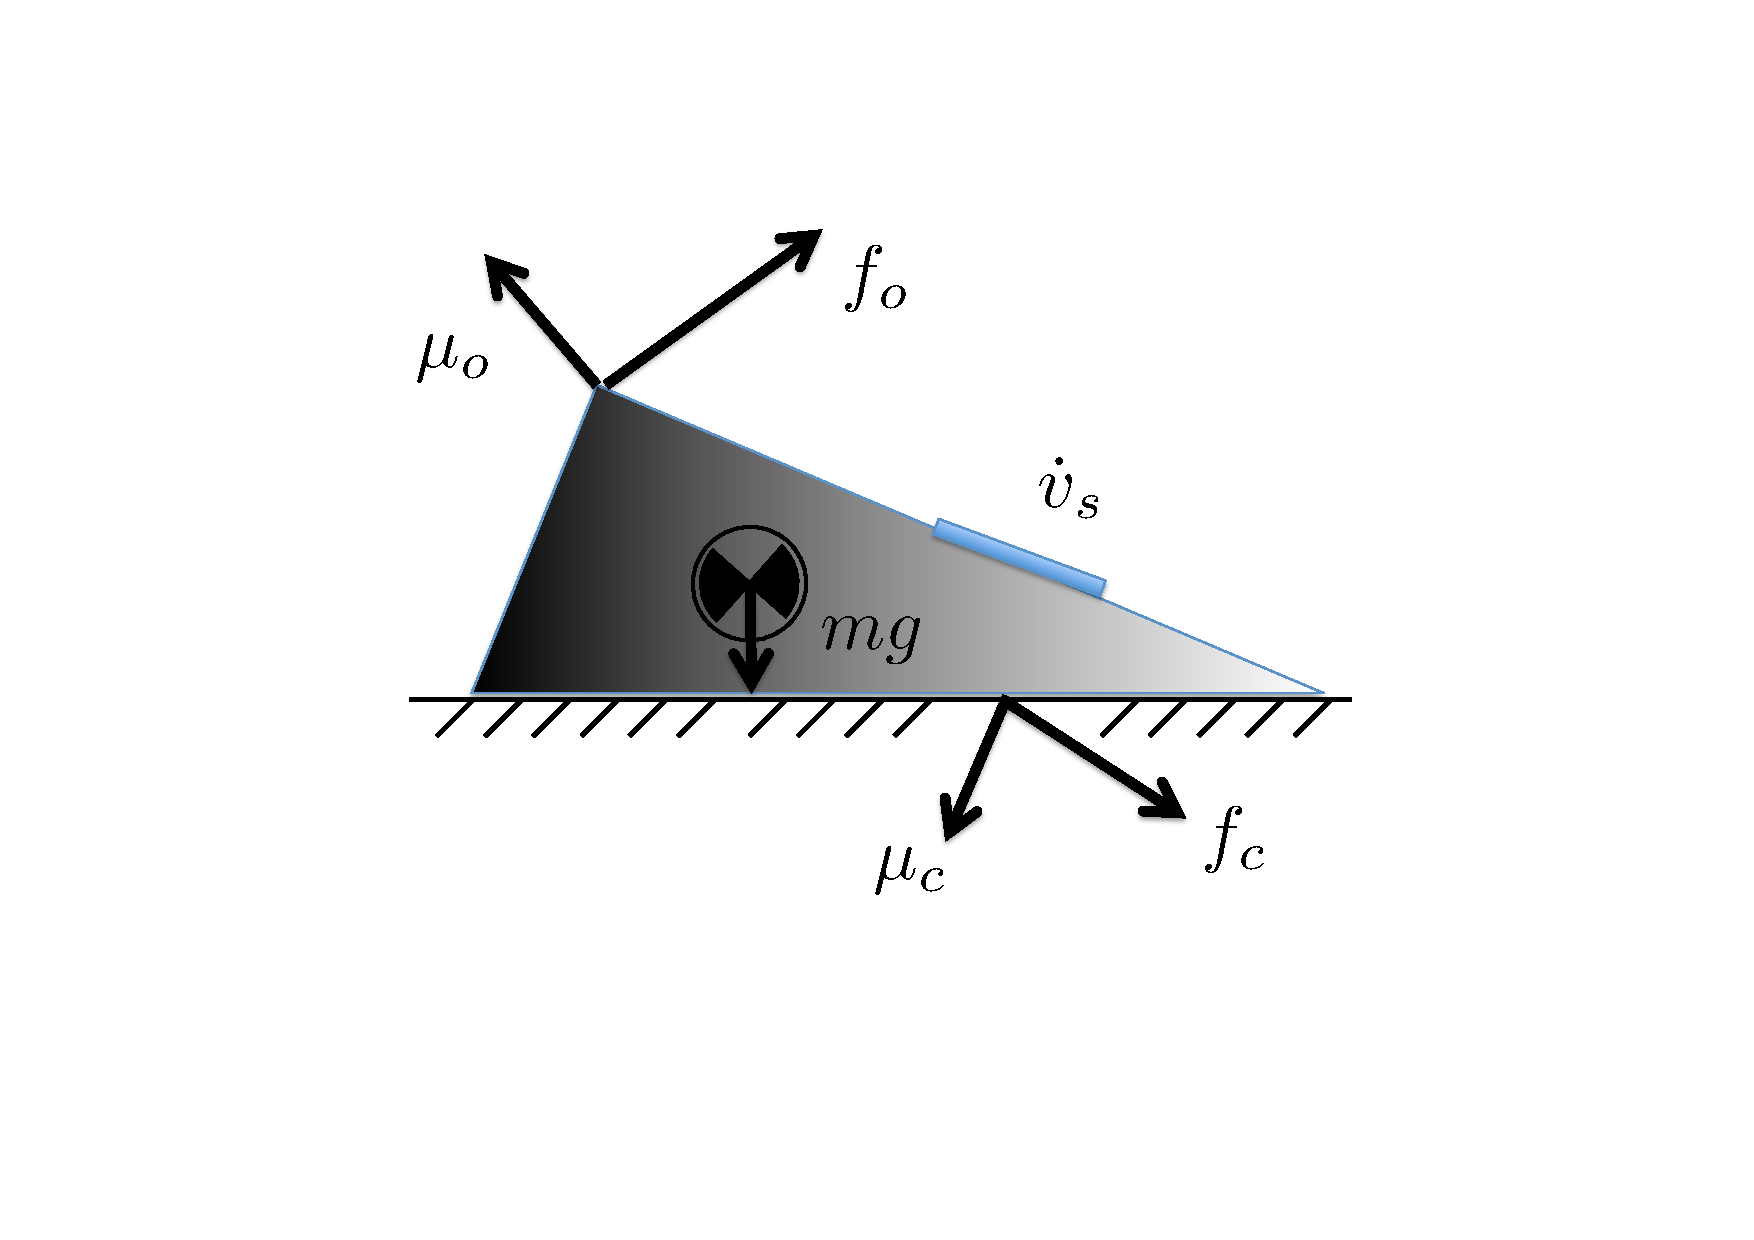
\includegraphics[width=0.35\textwidth]{./figs/foot.pdf}
    \caption{The foot of a bipedal robot as a rigid body. Two external wrenches can be considered - those applied at the ankle from the rest of the robot dynamics and the contact forces due to ground reaction.}
    \label{fig:foot_rigid_body}
\end{figure}

Consider the foot in contact with the ground as a single rigid body (see Fig. \ref{fig:foot_rigid_body}) subject to external wrenches with the following dynamics,

\begin{align}
 \begin{split}
  m \dot{v}^B + \omega^B \times (mv^B)              &= {f_o}^B + {f_c}^B + mg^B \\
  I^B\dot{\omega}^B + \omega^B \times (I^B\omega^B) &= {\mu_o}^B + {\mu_c}^B\\
  \dot{\phi}^B &= T_{\phi}^{-1} \omega^B
 \end{split}
\label{eq:dynamics}
\end{align}

where linear and angular velocities are given by $v^B$ and $\omega^B$. The external wrenches affecting the body are $({f_c}^B \quad {\mu_c}^B)$ and $(f_o^B \quad \mu_o^B)$. The first corresponds to the total wrench due to the body and control dynamics while the latter is due to contacts (as seen in Fig. \ref{fig:foot_rigid_body}). The superscript $*^B$ denotes quantities that are expressed in the body reference frame. The foot can be considered to have mass $m$ and inertia $I^B$. In the dynamics we have included also the orientation of the foot $\phi$, expressed in ZYZ Euler angles, or roll ($\alpha$), pitch ($\upsilon$) and yaw ($\psi$), since it will also be estimated. Its dynamics come from the relationship between the angular velocity $\omega$ and the rotational velocity $\dot{\phi}$ \cite{siciliano2009robotics} through the matrix 

\begin{equation}
T_{\phi} = \left[ \begin{array}{ccc}
                    0  &  -sin(\alpha)  &  cos(\alpha)sin(\upsilon)\\
                    0  &   cos(\alpha)  &  sin(\alpha)sin(\upsilon)\\
                    1  &       0        &  cos(\upsilon)                    
                   \end{array} \right]
\end{equation}

This local parametrization of the orientation is acceptable to reduce the complexities of using more consistent representations for the orientation, such as quaternions, since for the interest of the authors and the scope of the experiments later presented, the foot pitch is kept within $0<\upsilon<\pi$ thus avoiding singularities in the inversion of $T_{\phi}$.

From the dynamic model described in (\ref{eq:dynamics}), the state of our system is given by:

\begin{equation}
 x' = \left[ \begin{array}{c}
      v^B\\
      \omega^B\\
      \phi^B
     \end{array} \right]
     \label{eq:systemState}
\end{equation}

Inputs to this system are $u = [f_0^B \quad \mu_0^B \quad f_c^B \quad \mu_c^B]$. For the EKF, however, the state vector will be augmented to include these inputs and provide their estimates, so that (\ref{eq:systemState}) turns into: 

\begin{equation}
 x = [ v^B \quad \omega^B \quad f_o^B \quad \mu_o^B \quad fc^B \quad \mu_c^B \quad \phi^B]^T 
\end{equation}

We will then assume the following measurement vector:

\begin{equation}
  y = [f_o^B \quad \mu_o^B \quad f_c^B  \quad \mu_c^B \quad \dot{v}^B]^T 
\end{equation}

With the previously defined state and measurement vectors, the EKF can be computed as explained in Section \ref{subsection:extended-kalman-filter} in a recursive way, thus having at each time step $k$ an estimate of the external wrenches acting on the rigid body and an estimate of their covariances which can later be used to compute stability indices such as FRI and CoP. The way do this is described next. 

\subsection{Linearized stability indices}
Two kinds of stability indices were used and compared in this paper: FRI and CoP. The way to compute them used in this paper is described in \cite{Goswami99footrotation}. The equations for these measurements come from the static equilibrium equations of the foot at the desired stationary reference points (i.e. FRI or CoP), assuming that the dynamics of the rest of the body can be replaced by a F/T measurement at the ankle. For the CoP ($P$) the equation is

\begin{equation}
 \mu_c + PG \times m g - \mu_o - PO \times f_o = 0
 \label{eq:footBalance}
\end{equation}

Where $f_c$ and $\mu_c$ are assumed to be at the CoP of the single foot. $G$ is the reference frame of the foot center of mass (COM) and $O$ the ankle reference frame. Considering the tangential components $(.)_t$ of the previous equation yields the expression for the CoP, 

\begin{equation}
 (\mu_o + PO \times f_o - PG \times m g)_t = 0
 \label{eq:CoP}
\end{equation}

Changing the stationary reference point to one outside the support polygon and calling this point $F$, we obtain the expression for the FRI,

\begin{equation}
  (\mu_0 + FO \times f_o - FG \times m g)_t = 0
  \label{eq:FRI}
\end{equation}

At the point $F$, the resultant moment of the force and torque at the ankle plus the weight of the foot (different from the reaction forces) is normal to the surface.

To compute FRI and CoP after estimates of the external wrenches acting on the rigid body along with their corresponding variances, we simply express both external wrenches in the rigid-body frame (foot frame) and eliminate $PG$ from the equations. Solving for the $x$ and $y$ components of $P$ and $F$, the following simpler nonlinear relationships can be obtained. 
% \begin{equation}
%  \left[ \begin{array}{c} P_x  \\  P_y                  
%                    \end{array} \right] = \left[ \begin{array}{c}
%                     \frac{-{\mu_c}^x}{{f_c}^z}  \\
%                     \frac{{\mu_c}^y}{{f_c}^z} \end{array} \right] ,\quad  \left[ \begin{array}{c} F_x  \\  F_y                  
%                    \end{array} \right] = \left[ \begin{array}{c}
%                     \frac{-{\mu_o}^x}{{f_o}^z}  \\
%                     \frac{{\mu_o}^y}{{f_o}^z} \end{array} \right]                    
%   \end{equation}

  \begin{equation}
  \begin{split}
  P_x = \frac{-\mu_c^x}{f_c^z} &, \quad P_y = \frac{\mu_c^y}{f_c^z}, \\
  F_x = \frac{-\mu_o^x}{f_o^z} &, \quad F_y = \frac{\mu_o^y}{f_o^z},
  \end{split}
\end{equation}

\added[id=jeg]{NAVEEN Don't forget to add a few lines about how to fuse the estimates to get the corresponding estimate of the FRI and CoP along with their variances}


%... \added[id=jeg]{NAVEEN you can continue here explaining the procedure you followed}

% fLin     = - S(omega_B) * (m   * v_B    ) +  f_B_t_1 + f_B_t_2 + m*g.*R*[0; 0; 1];
% fAng     = - S(omega_B) * (I_B * omega_B) +  mu_B_t_1 + mu_B_t_2;
% df_B_1   =   u_t;
% df_B_2   =   u_t; %zeros(length(u_t),1);
% dmu_B_1  =   0.5*v_t;
% dmu_B_2  =   0.5*v_t; %zeros(length(v_t),1)
% dphi     =   inv(R)*omega_B;

%%%%%%%%%%%%%%%%%%%%%%%%%%%%%%%%%%%%%%%%%%%%%%%%%%%%%%%%%%%%%%%%%%%%%%%%%%%%%%%%%%
\section{EXPERIMENTS AND RESULTS}
\label{section:experiments}


\subsection{Simulation of a rigid body system}
% \added[id=jeg]{JORHABIB will take care of this using the last working version of the simulation}

The first set of experiments were carried out in simulation. The simulated rigid body was subjected to two wrenches. In order for these wrenches not to put the body in orientation singularity, an inverse dynamics algorithm was used to obtain suitable control inputs given a desired orientation trajectory. Afterwards, forward dynamics were integrated to simulate the evolution of the state vector $x$ and later the simulated outputs $y$. Noise was then added to implement the EKF. The parameters in Table \ref{table:simuParams} have been used for the simulations in Fig. \ref{fig:estimatedForces}-\ref{fig:estimatedOrientation}.

\begin{table}[h]
\caption{Simulation parameters}
\centering
\begin{tabular}{ccl}
\hline \hline
Parameter                   & Value        & Description \\ \hline \hline
$T$                         & 1.5 $s$      & Simulation time span\\
$\sigma_{v_f}$              & 0.025        & Forces meas. error variance\\
$\sigma_{v_u}$              & 0.025        & Torques meas. error variance \\
$\sigma_{v_a}$              & 0.01         & Lin. acc. meas. error variance\\
$\sigma_{v_{\omega}}$       & 0.01         & Ang. vel. meas. error variance\\
$\sigma_{w_f}$              & 0.04         & Forces error variance\\
$\sigma_{w_u}$              & 0.04         & Torques error variance\\
$\sigma_{w_a}$              & 0.001        & Lin. acc. error variance\\
$\sigma_{w_{\phi}}$         & 0.001        & Orientation error variance \\ 
$m$                         & 7 $Kg$       & Mass \\ 
$g$                         & 9.8 $m/s^2$  & Gravity\\ 
$\Delta t_{\textrm{EKF}}$   & 0.01 $s$     & Time interval used in EKF\\
$I_{xx}$                    & 0.05 $Kg \cdot m^2$& Main moment of inertia along x \\ 
$I_{yy}$                    & 0.02 $Kg \cdot m^2$& Main moment of inertia along y \\
$I_{zz}$                    & 0.03 $Kg \cdot m^2$& Main moment of inertia along z \\
\hline
\end{tabular}
\label{table:simuParams}
\end{table} 

The \emph{EKF/UKF Toolbox for Matlab} detailed in \cite{ekfToolbox} was used for the EKF algorithms.

\begin{figure}[t!]
 \centering
 \includegraphics[width=0.5\textwidth]{./figs/estimatedForces.eps}
 % estimatedForces.png: 656x660 pixel, 90dpi, 18.52x18.63 cm, bb=0 0 525 528
 \caption{Estimated external forces acting on the rigid body system after simulation.}
 \label{fig:estimatedForces}
\end{figure}

\begin{figure}[t!]
 \centering
 \includegraphics[width=0.5\textwidth]{./figs/estimatedTorques.eps}
 % estimatedForces.png: 656x660 pixel, 90dpi, 18.52x18.63 cm, bb=0 0 525 528
 \caption{Estimated external torques acting on the rigid body system after simulation.}
 \label{fig:estimatedTorques}
\end{figure}

\begin{figure}[t!]
 \centering
 \includegraphics[width=0.5\textwidth]{./figs/estimatedVelocities.eps}
 % estimatedForces.png: 656x660 pixel, 90dpi, 18.52x18.63 cm, bb=0 0 525 528
 \caption{Estimated angular and linear velocities of the rigid body system after simulation.}
 \label{fig:estimatedVelocities}
\end{figure}

\begin{figure}[t!]
 \centering
 \includegraphics[width=0.5\textwidth]{./figs/estimatedOrientation.eps}
 % estimatedForces.png: 656x660 pixel, 90dpi, 18.52x18.63 cm, bb=0 0 525 528
 \caption{Estimated orientation $\phi(t) = [\alpha \quad \upsilon \quad \psi]^T$ during simulation.}
 \label{fig:estimatedOrientation}
\end{figure}

\subsection{Implementation on the real platform}
% \added[id=nav]{NAVEEN could give me a hand here describing the experiments and putting the corresponding graphs. We should describe the whole setup and draw some sort of diagram explaining each part of it, e.g. wholeBodyDynamicsTree, MATLAB Toolbox, etc.}
% \added[id=jeg]{JORHABIB I can draw some sort of block diagram explaining the entire system}

The iCub robot was used for the experiments described in this section. We used two sets of force/torque measurements and an external measurement of acceleration and angular velocity (using a Vicon tracker system). The scenario tested was that of externally induced toppling. The aim was to estimate accurately the variation in the stability indices (CoP, FRI) during the momments preceding and at toppling. 

The F/T sensors used for the experiment are depicted in Fig. \ref{fig:icub_ft_sensors}. 

The scenario tested was to predict the behaviour of the stability indices, particularly that of the CoP as the robot reaches a toppling condition.  F

The robot was placed in a standing-upright position with knees Toppling was induced by rotating the torso of the robot in the saggital plane, i.e. bending forward. The topling condition expected is that the CoP exits the support polygon at the momment of toppling.

The parameters used in the experiments with the robot can be found in Table \ref{table:paramsPlatform}

\begin{table}[h]
\caption{Parameters for experiment on the real platform \added[id=jeg]{NAVEEN Don't forget to fill in this table.}}
\centering
\begin{tabular}{ccl}
\hline \hline
Parameter                   & Value        & Description \\ \hline \hline
$T$                         &  $s$      & Simulation time span\\
$\sigma_{v_f}$              &         & Forces meas. error variance\\
$\sigma_{v_u}$              &         & Torques meas. error variance \\
$\sigma_{v_a}$              &          & Lin. acc. meas. error variance\\
$\sigma_{v_{\omega}}$       &          & Ang. vel. meas. error variance\\
$\sigma_{w_f}$              &          & Forces error variance\\
$\sigma_{w_u}$              &          & Torques error variance\\
$\sigma_{w_a}$              &         & Lin. acc. error variance\\
$\sigma_{w_{\phi}}$         &         & Orientation error variance \\ 
$m$                         &  $Kg$       & Mass \\ 
$g$                         & 9.8 $m/s^2$  & Gravity\\ 
$\Delta t_{\textrm{EKF}}$   &  $s$     & Time interval used in EKF\\
$I_{xx}$                    &  $Kg \cdot m^2$& Main moment of inertia along x \\ 
$I_{yy}$                    &  $Kg \cdot m^2$& Main moment of inertia along y \\
$I_{zz}$                    &  $Kg \cdot m^2$& Main moment of inertia along z \\
\hline
\end{tabular}
\label{table:paramsPlatform}
\end{table} 

\begin{figure}[t!]  
  \centering
    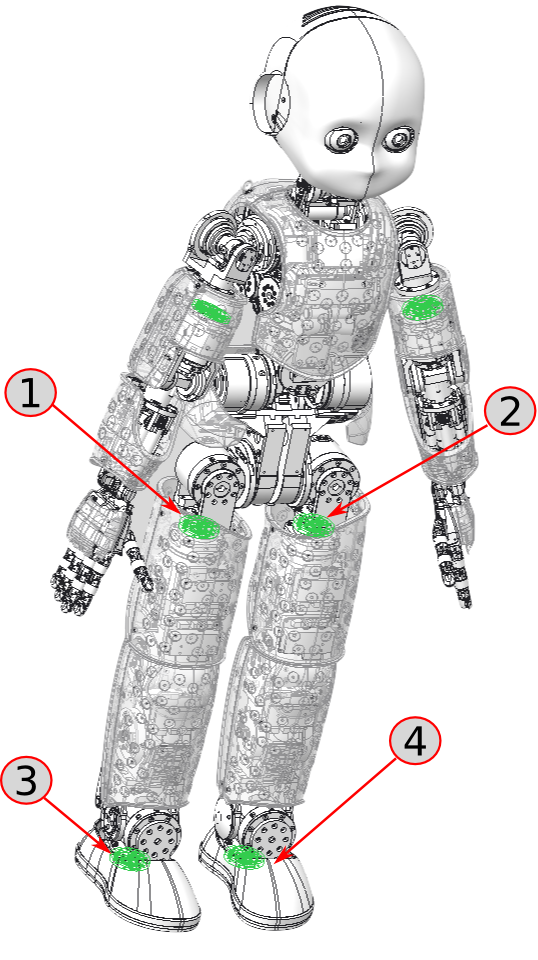
\includegraphics[width=0.25\textwidth]{./figs/icub_force_selected.png}
    \caption{Schematic of iCub and the force/torque sensors used for the experiments. 
    \label{fig:icub_ft_sensors}}
\end{figure}


%%%%%%%%%%%%%%%%%%%%%%%%%%%%%%%%%%%%%%%%%%%%%%%%%%%%%%%%%%%%%%%%%%%%%%%%%%%%%%%%%%
\section{CONCLUSIONS}
% \added[id=jeg]{JORHABIB will contribute here} \added[id=nav]{NAVEEN will contribute here} \added[id=fra]{FRA will contribute here}
% \added[id=jeg]{We need to elaborate on the importance of the work, suggest applications and extensions}
\label{section:conclusions}

%%%%%%%%%%%%%%%%%%%%%%%%%%%%%%%%%%%%%%%%%%%%%%%%%%%%%%%%%%%%%%%%%%%%%%%%%%%%%%%%%%
\section{FUTURE WORK}
\label{section:futureWork}
Equation (\ref{eq:dynamics}) can easily be generalized for rigid bodies with $N$ external wrenches, for which the method we use in this paper could indeed be seen as a framework for the estimation of dynamic quantities including the inputs to the system. In the future we would like to expand this estimation process to any contact point in the structure. For a robot like iCub, we can still obtain this sort of measurements, since it is fully endowed with a sensorized skin containing also embedded accelerometers. For whole body estimations however, the estimates of the orientation of the different rigid bodies would be highly affected by the kind of parametrization that has been used in this paper, since for other parts of the body the probability of falling in orientation singularities becomes higher. For this reason, a better representation of orientation would be necessary. A quaternion based Extended Kalman Filter is seen as a viable solution taking inspiration from aircraft control approaches. The additional hardware effort would be represented by the addition of distributed gyroscopes to simplify the dynamic modeling as done in \cite{roumeliotis1999}. Finally, to allow for real-time performance, the computationally expensive update stage of the EKF can be improved with a Bayesian Network approach in which $x_{k|k}$ can be estimated given $y_k$, thanks to the sparsity of the resulting measurement matrix of the linearized measurement model.  

% \added[id=jeg]{JORHABIB Here I shouldn't forget to write about how to make computations faster by using a bayesian network to perform the prediction stage as well as the use of quaternions for the reasons explained in the wiki of this repository.}

%\bibliographystyle{IEEEtran}
\bibliographystyle{abbrv}
\bibliography{estimationRefs}


\end{document}
